\documentclass[hidelinks, a4paper,twoside]{civiltools_report}
\usepackage{array, boldline, makecell, booktabs}
\newcommand\btrule[1]{\specialrule{#1}{0pt}{0pt}}
\usepackage{colortbl}
\usepackage{multicol,caption}               % three-column layout
\usepackage[font={footnotesize}]{caption}
\usepackage{xcolor}
\usepackage{amsmath}
% \usepackage{ae}
\usepackage{geometry}
\usepackage{multirow}
\usepackage{siunitx}
\usepackage[title]{appendix}
\usepackage{longtable} 
\usepackage{hyperref}
\usepackage{flafter}
\usepackage{afterpage}
\usepackage{varioref}
% \usepackage[utf8]{inputenc}
\usepackage{graphicx}
\usepackage{setspace}
\setstretch{2}
\usepackage[many]{tcolorbox}
\usepackage{float}
\usepackage{xcolor}
\hypersetup{
    colorlinks,
    linkcolor={blue!70!black},
    citecolor={blue!50!black},
    urlcolor={blue!80!black}
    }
\usepackage{xepersian-multiplechoice}
\usepackage{xepersian}
\settextfont[Scale=1.4]{XB Niloofar}
% \setlatintextfont[Scale=1.3]{Times New Roman}
%\usepackage{draftwatermark}
%\SetWatermarkText{Draft}
%\SetWatermarkScale{1}

% \newenvironment{Figure}
%   {\par\medskip\noindent\minipage{\linewidth}}
%   {\endminipage\par\medskip}

  
% \title{دفترچه محاسبات سازه}
% \newcommand{\punch}{نرم افزار برش پانچ}
% \newcommand{\address}{شهرک شکوهیه فاز 2 خ بابایی خ تهرانی مقدم نبش فرعی 5}
% \author{ابراهیم رعیت رکن آبادی}
% % \date{}
% \today{}

%\vspace{3cm}\textbf{NOTE: This preliminary  report is simply deemed suitable for the purpose of pre-dimensioning the structures addressed and obtaining the loads transmitted by them upon the foundation. The equipment modelling doesn't reflect its final geometric characteristics.}}
% \renewcommand{\revision}{1.0}

\begin{document}
% \begin{center}
%   بنام خدا \newline
%   \maketitle
%   \vspace{10cm}
%   مالک: شرکت سلامت گستران پردیس پارت
%   \newline
%   پلاک ثبتی:
% \end{center}


% \newpage
% \renewcommand{\abstractname}{Executive Summary}.
% \maxdeadcycles=200

% %\maketitle
% \tableofcontents
% \listoftables
% \listoffigures
% \newpage
\pagenumbering{Roman}    % a, b, c, ...
\thispagestyle{empty}
% نحوه درج کردن لوگوی دانشگاه
\begin{figure*}[!h]
\centerline{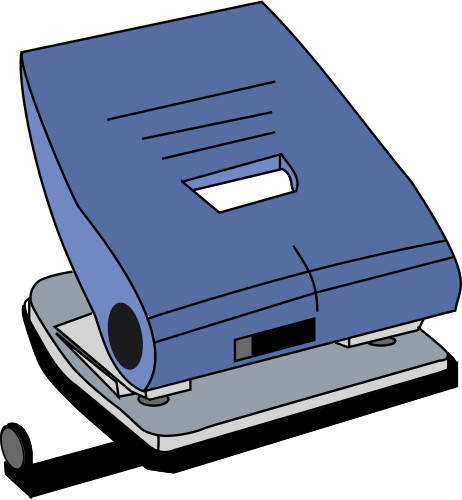
\includegraphics[width=4cm]{logo}}
%\caption{}
\end{figure*}
\begin{center}
%دستوری برای کم کردن فاصله بین لوگو و خط پایین آن
\vspace{-.8cm}

% {\large پژوهشگاه بین المللی زلزله شناسی و مهندسی زلزله}
%دستوری برای تعیین فاصله بین دو خط


\\[1cm]
بنام خدا
\\[1cm]
راهنمای کاربری
\\[.8cm]
% {\nastaliq
\begin{Huge}
نرم افزار 
\lr{CivilTools}
\end{Huge}

\\[.5cm]
\begin{latin}
    \textbf{Ver. 5.0}
\end{latin}



\begin{figure}[ht]
    \centering
        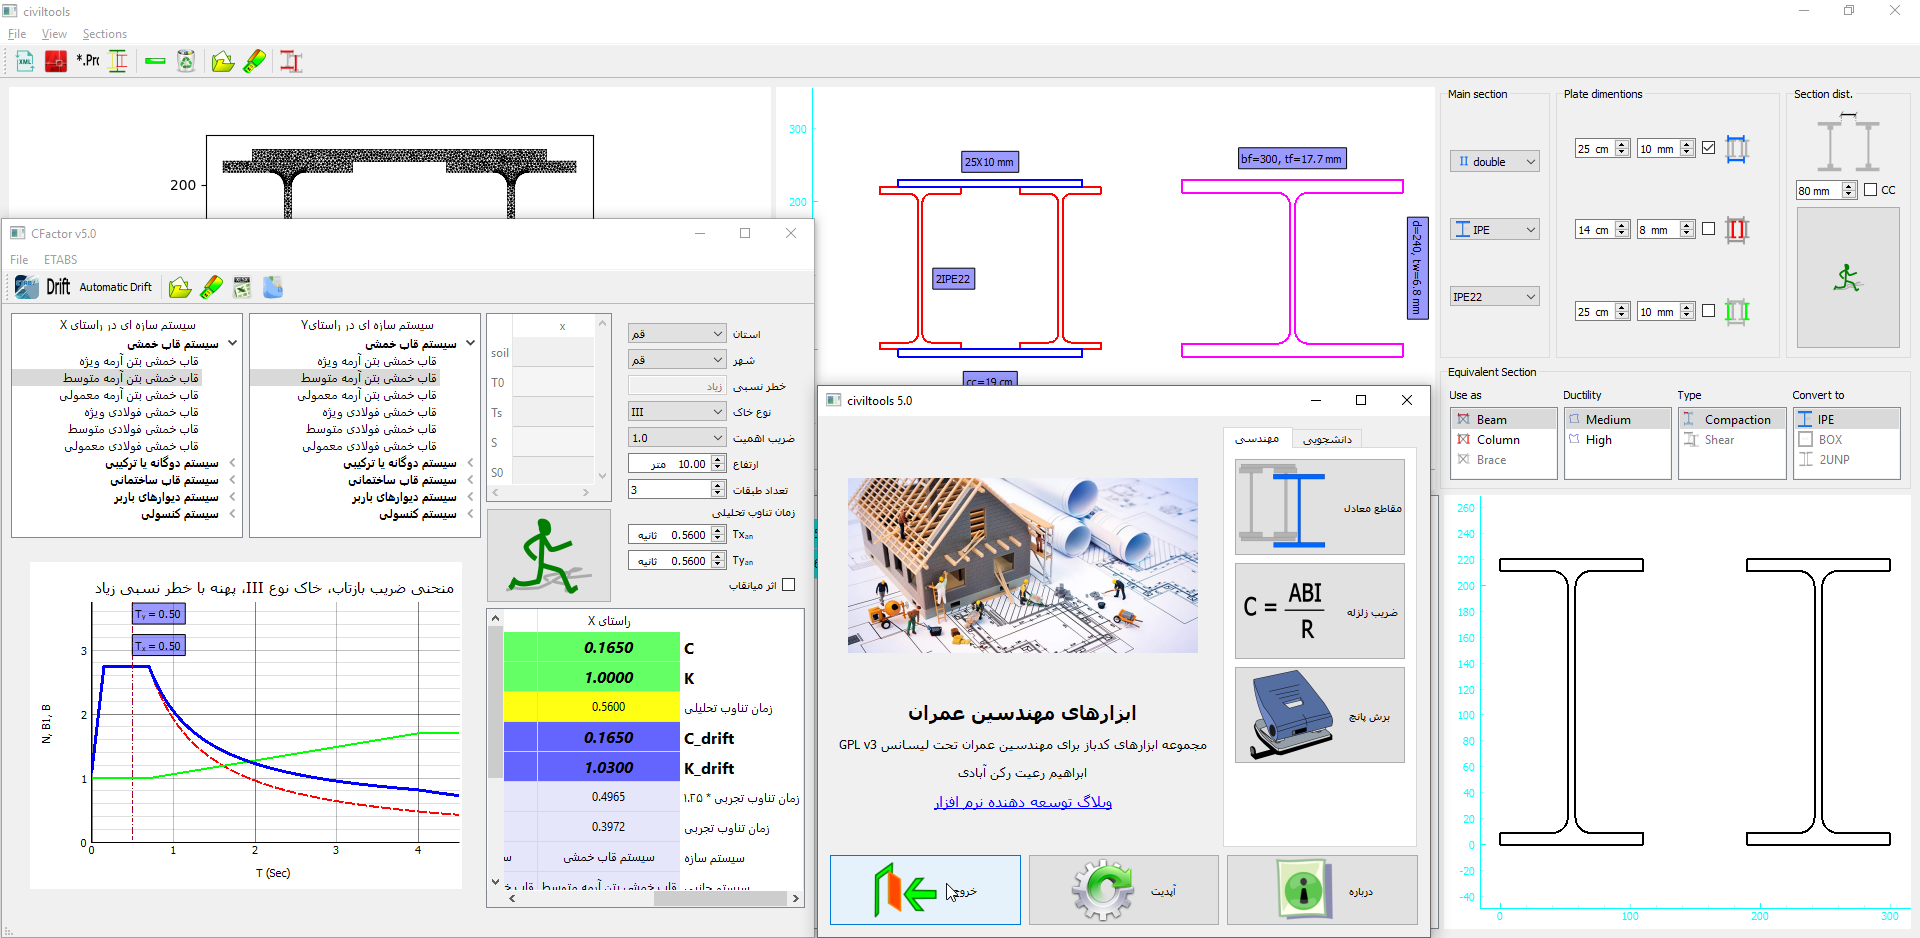
\includegraphics[width=\linewidth]{figures/civiltools}
        % \caption{DL, units:[m,kN]}
        % \label{dl-unitsmkn}
\end{figure}

\\[2.5cm]{ توسعه دهنده:}
\\[.3cm]
\textbf{{\large  \developer}}

% \\[2cm]{کارفرما}
% \\[.3cm]
% \textbf{{\large \karfarma}}
% \\ \textit{\address}

\\[1.cm]
\today
\end{center}
%\maketitle
%دستوری برای رفتن به صفحه جدید
\newpage
\thispagestyle{empty}
% \pagenumbering{Roman}   % i, ii, iii, iv, ...
\setcounter{page}{1}
\tableofcontents
% \listoffigures
% \listoftables
\newpage

\pagenumbering{arabic}
\section*{مقدمه}

با عرض سلام خدمت مهندسین گرامی \newline
اواخر دوره کارشناسی، علاقه زیادی به سیستم های کامپیوتری و مخصوصا سیستم عامل لینوکس پیدا کردم. بعد از آشنایی با لینوکس با فلسفه نرم افزارهای کدباز آشنا شدم و خیلی مجذوب این فلسفه شدم.
برخلاف ویندوز و خیلی از نرم افزارهای دیگر که کدبسته هستند، کد نوشته شده برای نرم افزارهای کدباز در دسترس عموم قرار دارد. این یعنی هر کسی میتواند به کدهای نرم افزار دسترسی داشته باشد و آنها را خوانده و یا حتی مطابق با نیاز خود در آن تغییرات ایجاد کند. 
من هم تصمیم گرفتم که به این فلسفه بپیوندم و مشکلات نرم افزاری که مهندسین عمران با آن برخورد میکنند را به مرور زمان و در حد توان با ایجاد نرم افزارهای کدباز، کمتر و یا حذف نمایم. نرم افزار حاضر که متشکل از دو نرم افزار اصلی مقاطع معادل و ضریب زلزله و تعدادی نرم افزار دانشجویی است
حاصل این کار است. امیدوارم که مهندسین عزیز بتوانند از آنها استفاده کنند و نیازهای خود را برطرف نمایند.
در صورتی که نظر یا پیشنهادی در مورد نرم افزارها داشتید از طریق تلگرام و یا ایمیل با من در میان بگذارید.



کانال تلگرام: \lr{@civiltools} \newline
آی دی تلگرام: \lr{@roknabadi} \newline
ایمیل: \lr{ebe79442114@yahoo.com, ebe79442114@gmail.com}

\newpage
% \begin{twocolumn}
\section{نرم افزار محاسبه ضریب زلزله (\lr{CFactor})}

\begin{figure}[H]
    \centering
    
\includegraphics[scale=.6]{figures/cfactor}
    \caption{صفحه اصلی نرم افزار محاسبه ضریب زلزله}
\end{figure}
توسط این نرم افزار کاربر میتواند ضریب زلزله را مطابق با ویرایش چهارم آیین نامه ۲۸۰۰ بدست آورد. علاوه بر این امکانات دیگری هم در این نرم افزار گنجانده شده که انشالله به مرور زمان تکمیل خواهد شد. ویژگی های کلی

\begin{itemize}
    \item اعمال ضریب زلزله در فایل ایتبز
    \item محاسبه ضریب زلزله دریفت
    \item ساخت فایل طیف طراحی
    \item کنترل دریفت
    \item محاسبه خودکار دریفت
    \item بررسی نامنظمی پیچشی
    \item نمایش برش طبقات
    \item کنترل خودکار معیار مقاومت طبقه
    \item کنترل نامنظمی جرمی
    \item کنترل طبقه نرم
\end{itemize}

تمامی این ویژگی ها بر روی ایتبزهای ورژن 2018 و 2019 کار میکند و در مورد ایتبز 2016 و پایینتر کارایی ندارند. زیرا از نسخه 2018 به بعد نرم افزار ایتبز، 
توابع 
\lr{API}
این نرم افزار پایدار شده اند و با کمترین مشکل کار خواهند کرد، گرچند که هنوز هم نواقص بسیاری دارد.
گاهی اوقات در بعضی از فایل ها این توابع به صورت ناقص اجرا میشود که باعث خرابی فایل میشود، 

\textcolor{red}{لذا همیشه قبل از استفاده از قابلیت های فوق، یک بک آپ از فایل خود بگیرید.}

\subsection{اعمال ضرایب زلزله در فایل ایتبز}
در حال حاضر امکانات مربوط به ایتبز برای ایتبزهای ۲۰۱۸ به بعد کار میکند. برای این منظور بعد از محاسبه ضریب زلزله و زمانیکه فایل ایتبز باز است، از منوی
$ETABS \rightarrow Export to Etabs$
برای اعمال ضریب زلزله در فایل ایتبز استفاده کنید. اگر سازه در حالت تحلیل شده قرار داشته باشد، نرم افزار به طور خودکار قفل آنرا باز میکند و سپس ضرایب زلزله را در فایل ایتبز اعمال میکند.

\begin{itemize}
    \item نرم افزار به طور خودکار جهات \lr{X, Y} و همچنین زلزله های دریفت را تشخیص میدهد.
    \item گاهی اوقات در بعضی از فایلها این کار به درستی صورت نمیگیرد. اگر بعد از اعمال ضریب زلزله، نتوانستید فایل را اجرا کنید، نگران نباشید. فایل را بسته و دوباره باز کنید. هنوز به طور دقیق علت این ایراد را متوجه نشده ام، در صورت برخورد با این مشکل فایل را برای من ارسال کنید تا مشکل اینگونه فایل ها را بررسی کنم.
\end{itemize}

\subsection{محاسبه ضریب زلزله دریفت}
با توجه به زمان تناوب های تحلیلی سازه که توسط کاربر وارد میشود، نرم افزار اقدام به محاسبه ضریب زلزله دریفت مینماید. 

\subsection{ساخت فایل طیف طراحی}
فایلهای آماده زیادی برای وارد کردن طیف طراحی در نرم افزار ایتبز وجود دارد، ولی اکثر آنها تنها چند پارامتر را مدنظر قرار میدهند مثل نوع خاک و شتاب مبنای طرح، ولی با توجه به گستردگی سیستم های باربر جانبی که ضریب رفتارهای مختلفی دارند،
ساخت همه حالتهای طیف عملا غیرممکن و غیرضروری است. ولی نرم افزار ضریب زلزله یک طیف مختص به سازه انتخاب شده برای شما ایجاد میکند که دیگر نیاز به اعمال هیچ گونه ضریبی در موقع ساخت
\lr{Load Case}
دینامیکی  در نرم افزار ایتبز وجود ندارد.
کافی است که طیف ساخته شده را مطابق شکل 
\ref{pic:spec_scale}
بدون اعمال هیچ گونه ضریب در نرم افزار ایتبز وارد کنید.

\begin{figure}[H]
    \centering
    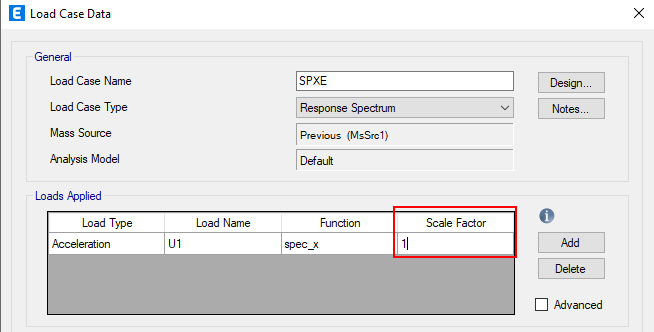
\includegraphics[scale=.7]{figures/spec_scale.png}
    \caption{نحوه ساخت حالت بار دینامیکی بدون نیاز به اعمال ضریب}
    \label{pic:spec_scale}
\end{figure}

همچنین در صورتی که سیستم های جهت 
\lr{X, Y}
متفاوت باشند نرم افزار به طور خودکار برای هر جهت یک طیف مجزا درست میکند. سپس میتوانید فایل آماده شده را مطابق شکل
\ref{pic:spec}
به نرم افزار معرفی نمایید.

\begin{figure}[H]
    \centering
    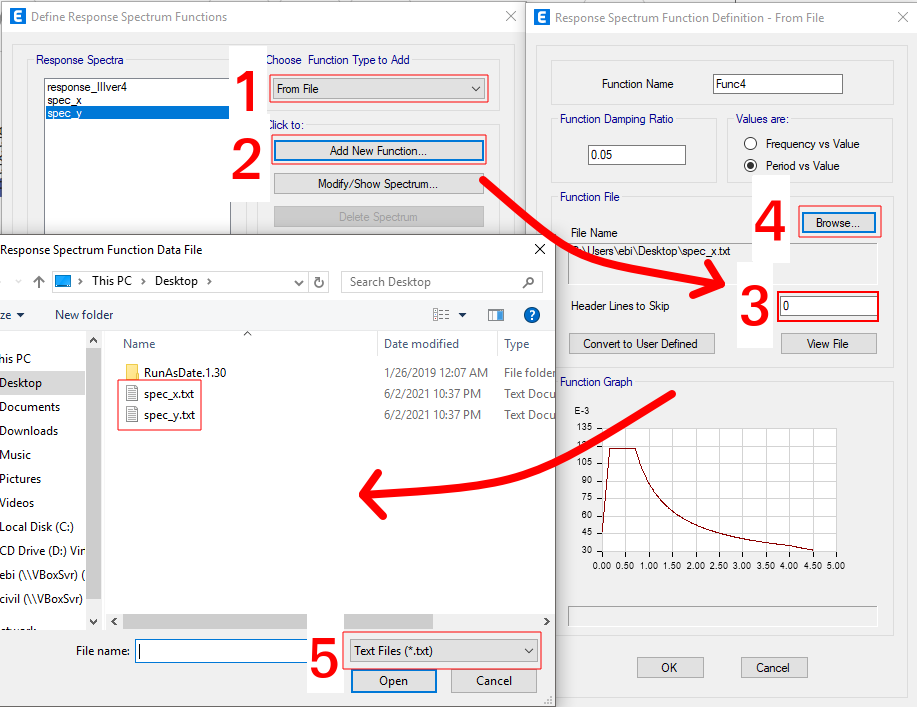
\includegraphics[scale=.6]{figures/spec}
    \caption{مراحل وارد کردن طیف به نرم افزار ایتبز}
    \label{pic:spec}
\end{figure}

\subsection{کنترل دریفت}
با استفاده از گزینه کنترل دریفت شما میتوانید با توجه به سیستم های باربر جانبی که انتخاب نموده اید و همچنین مشخص کردن تعداد طبقات سازه مقدار دریفت موجود و دریفت مجاز را برای هر راستا مشاهده کنید.
نرم افزار به طور خودکار زلزله های دریفت را تشخیص میدهد و مقادیر دریفت را برای آنها نمایش میدهد.  اگر پیغامی دریافت کردید که باید یک حالت بار یا همان 
\lr{Load Case}
انتخاب کنید، نشان دهنده این است که شما هیچ زلزله دریفتی تعریف نکرده اید.
با سرچ در کادر 
\lr{Filter}
با توجه به ستون انتخاب شده در گزینه 
\lr{By Column}
، میتوانید خروجی جدول را برای مشاهده بهتر فیلتر نمایید مثلا اگر مطابق شکل
\ref{pic:drift}
گزینه ستون را
\lr{OutputCase}
انتخاب کنید، با تایپ 
\lr{dri}
فقط دریفت هایی که در نام آنها \lr{dri} باشد نمایش داده میشوند.

\begin{figure}[H]
   \centering
   
\includegraphics[scale=0.7]{figures/drift}
   \caption{فیلتر کردن خروجی جدول دریفت با انتخاب ستون مربوطه و تایپ  مقداری از محتوای ستون}
   \label{pic:drift}
\end{figure}

همچنین با کلیک روی عنوان ستونها نیز میتوانید مطابق شکل 
\ref{pic:drift_filter}
 آنها را فیلتر نمایید. فیلتر فقط روی یک ستون اعمال میشود و نمیتوان همزمان فیلتر روی چند ستون اعمال نمود، یعنی با فیلتر نمودن یک ستون، فیلتر مابقی ستونها بی اثر میشود.
 
 
\begin{figure}[H]
    \centering
    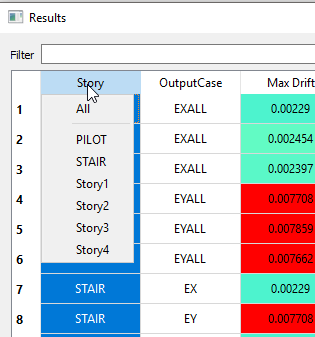
\includegraphics[scale=0.7]{figures/drift_filter}
    \caption{فیلتر کردن خروجی جدول دریفت با کلیک روی نام ستون ها}
    \label{pic:drift_filter}
\end{figure}


\subsection{محاسبه خودکار دریفت}
قبل از اجرای این دستور، کاربر باید سیستم های مقاوم باربر جانبی را به درستی انتخاب کند، زیرا نرم افزار مقادیر مجاز دریفت را بر اساس تعداد طبقات و مقادیر 
\lr{cd}
سیستم های انتخابی محاسبه میکند.

با کلیک روی گزینه 
\lr{Automatic Drift}
پنجره ای مطابق شکل \ref{pic:top_bot_story} نمایش داده میشود.
نرم افزار به طور خودکار طبقات پایین و بالای سازه را از روی فایل ایتبز تشخیص میدهد، در عین حال کاربر میتواند طبقات را تغییر دهد که با این کار تعداد طبقات و ارتفاع به طور خودکار از فایل ایتبز محاسبه میشود.
در نهایت کاربر به انتخاب خود میتواند تعداد طبقات و ارتفاع دلخواه را نیز وارد نماید.

\begin{figure}[H]
    \centering
    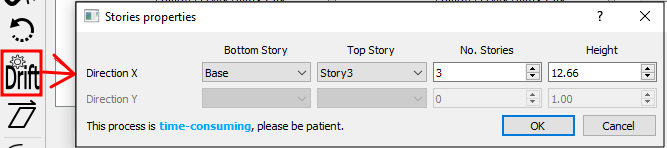
\includegraphics[scale=0.7]{figures/top_bot_story}
    \caption{مشخص کردن تعداد طبقات و ارتفاع سازه}
    \label{pic:top_bot_story}
\end{figure}

بعد از تایید کاربر، مراحل زیر انجام میگیرد:
\begin{itemize}
    \item ابتدا یک کپی از فایل اصلی به نام \lr{T.EDB} در محل فایل اصلی ساخته میشود.
    \item در این فایل ضرایب سختی خمشی تیرها و ستونها به ترتیب $0.5$ و $1.0$ قرار داده میشود.
    \item سازه آنالیز شده و مقادیر زمان تناوب تحلیلی در راستای \lr{x, y} استخراج میشود.
    \item ضریب زلزله و ضریب زلزله دریفت بر مبنای زمان تناوب تحلیلی مرحله قبل مجددا محاسبه میشود.
    \item سپس جدول دریفت بر اساس تعداد طبقات و سیستم های انتخابی کاربر مطابق شکل \ref{pic:drift} به نمایش در می آید.
\end{itemize}

\subsection{بررسی نامنظمی پیچشی}
از طریق منوی 
$ETABS \rightarrow Rho Factor \rightarrow Show Torsion$
میتوانید مقادیر پیچش طبقات را به صورت یک جدول مشاهده کنید. نرم افزار به طور خودکار نتایج نامعتبر را حذف میکند، به این معنی که زمانیکه نیرو در راستای 
\lr{x}
وارد میشود، مقادیر دریفت در راستای \lr{y} را حذف میکند و همین طور برعکس. این بدین دلیل است که گاهی اوقات مقادیر دریفت در راستایی که نیرو وارد نمیشود
بسیار کم است و زمانیکه مقادیر دریفت حداکثر و متوسط که اعداد کمی هستند در ایتبز بر هم تقسیم میشوند،‌ نسبت بزرگی میدهند مثل عدد ۳ یا ۴ که کاربر باید در ایتبز این
مقادیر را از نتایج حذف کند. نرم افزار به طور خودکار این نتایج را نمایش نمیدهد. در نهایت جدول پیچش مطابقه شکل 
\ref{pic:torsion}
با رنگ بندی نمایش داده میشود:

\begin{figure}[H]
    \centering
    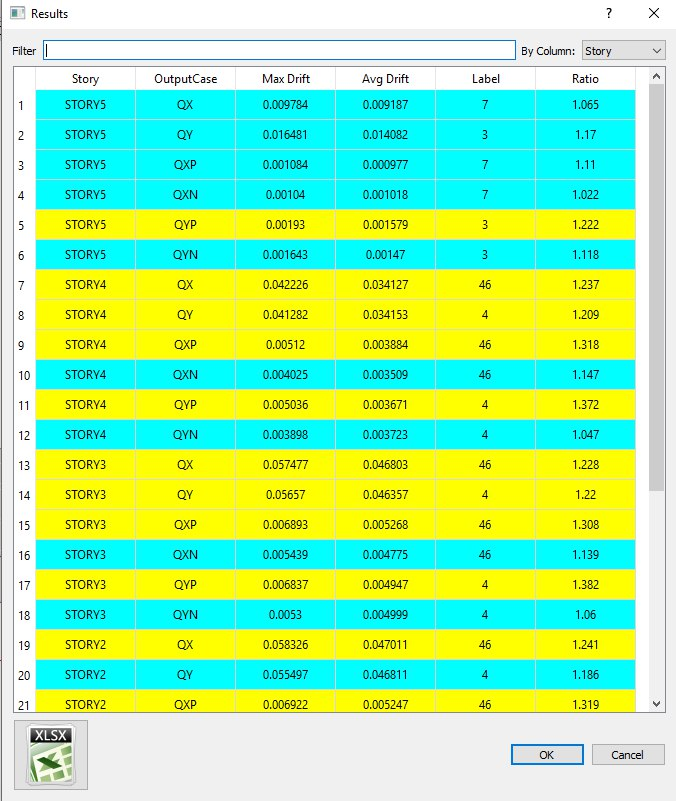
\includegraphics[scale=0.7]{figures/torsion_table}
    \caption{نمایش پیچش طبقات}
    \label{pic:torsion}
\end{figure}

همچنین با کلیک بر روی هر ردیف از جدول، مطابق شکل 
\ref{pic:torsion_show_node}
نقطه ای که کنترل پیچش روی آن صورت گرفته است به نمایش در می آید و کاربر میتواند کنترل کامل روی نقاطی
که نرم افزار ایتبز انتخاب کرده است داشته باشد.

\begin{figure}[H]
    \centering
    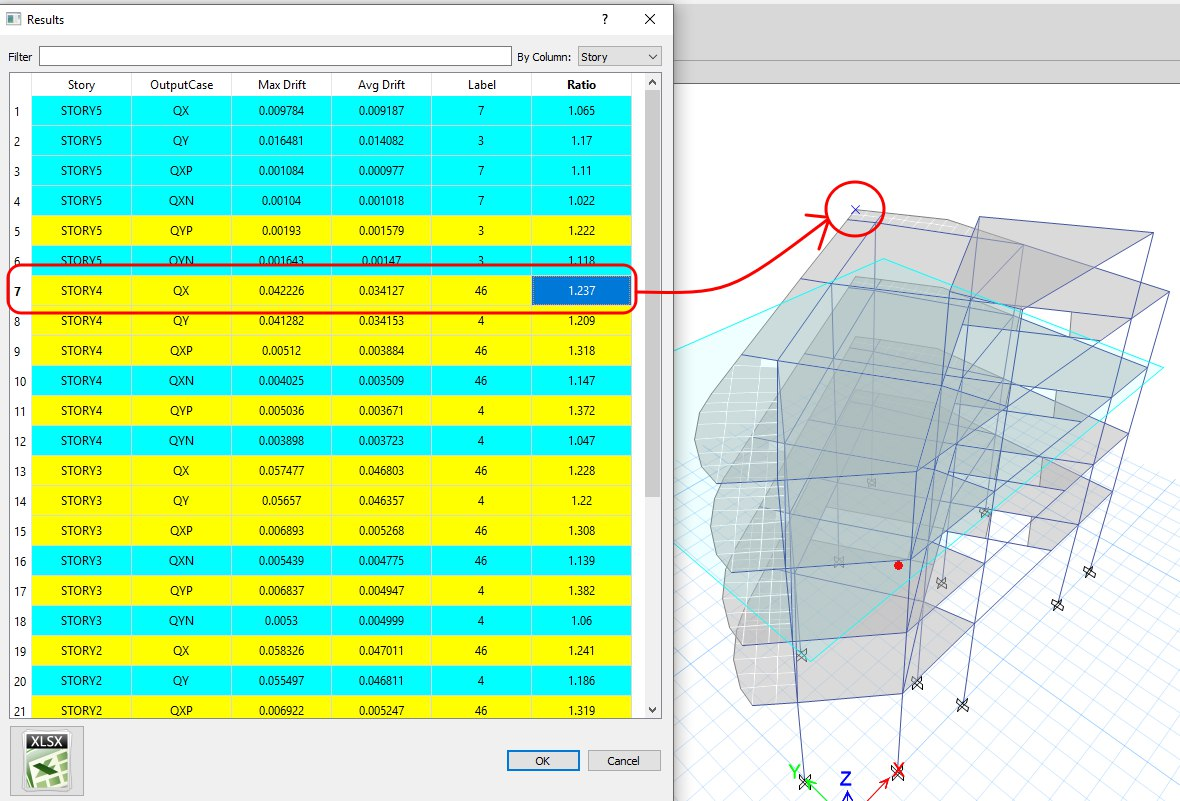
\includegraphics[scale=0.4]{figures/torsion_show_node}
    \caption{نمایش نقطه مورد نظر با کلیک روی ردیف های جدول}
    \label{pic:torsion_show_node}
\end{figure}

\subsection{نمایش برش طبقات}
یکی از کنترل هایی که در زمان محاسبه ضریب نامعینی مورد نیاز است، طبقاتی است که برش در آنها از $.35$ 
برش پایه تجاوز میکند. با انتخاب این گزینه از منوی 
$ETABS \rightarrow Rho Factor \rightarrow Story Forces$
جدول مقادیر برش طبقات به همراه رنگ بندی مناسب مطابق شکل 
\ref{pic:story_forces}
نمایش داده میشود. در این جدول نسبت نیروها در دو راستای
$x, y$
به صورت مجزا نمایش داده میشود و طبقاتی که به رنگ سبز هستند نیاز به کنترل ضابطه مربوطه را ندارند.

\begin{figure}[H]
    \centering
    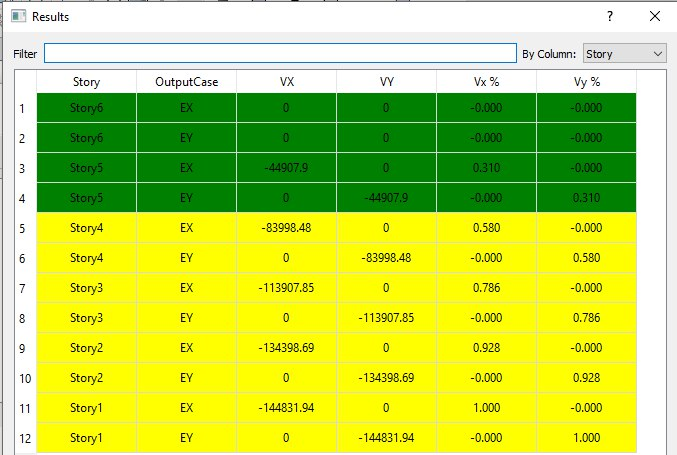
\includegraphics[scale=0.7]{figures/story_forces}
    \caption{نیروی برش طبقات و نسبت آنها به برش پایه}
    \label{pic:story_forces}
\end{figure}

نرم افزار برای تشکیل این جدول به طور خودکار یک زلزله  از زلزله های جهت 
$x$ و 
همینطور یک زلزله  از زلزله های جهت $y$
را میخواند، که میتواند با یا بدون خروج از مرکزیت باشد، زیرا برش طبقه ارتباطی به خروج از مرکزیت نیرو ندارد. در این موارد زلزله های دریفت به طور خودکار نادیده گرفته میشوند.


\subsection{کنترل خودکار معیار مقاومت طبقه}
یکی از مراحل دیگر در کنترل ضریب نامعینی کنترل مربوط به معیار مقاومت طبقه است. مراحل کار بدین صورت است:

\begin{itemize}
    \item ابتدا کاربر در نرم افزار ایتبز، تیری را که بیشترین اثر کاهش روی مقاومت طبقه دارد را انتخاب میکند. برای این کار میتوانید از مقدار انرژی داخلی عضو استفاده کنید.
    \item سپس کاربر از منوی $ETABS \rightarrow Rho Factor \rightarrow Get Weakness$ دستور را اجرا میکند.
    \item در صورتیکه سازه آنالیز و طراحی نشده باشد، نرم افزار سازه را آنالیز و طراحی میکند.
    \item سپس نتایج تیر و ستون طبقه ای که عضو انتخاب شده در آن قرار دارد استخراج میشود. در این مرحله نسبت تنش ستونها در ایستگاه حداکثر و مقادیر میلگردهای بالا و پایین و همینطور میلگرد برشی تیرها در ایستگاه های مختلف برداشت میشود.
    \item سپس یک کپی از فایل اصلی با نام \lr{weakness.EDB} در محل فایل اصلی ساخته میشود.
    \item در این فایل تیر انتخاب شده توسط کاربر دو سر مفصل میشود (خمش ابتدا و انتها و پیچش یک سمت تیر آزاد میشود).
    \item سپس ضرایب زلزله به صورت خودکار در مقدار$0.67$ ضرب میشوند.
    \item سازه تضعیف شده آنالیز و طراحی میشود.
    \item همانند فایل اصلی مقادیر نسبت تنش ستونها و مساحت میلگردهای طبقه مورد نظر برداشت میشود.
    \item سپس جدول نسبت تنش ستونها و مقادیر میلگردها مطابق شکل های \ref{pic:weakness_column} و \ref{pic:weakness_beam} به نمایش در می آیند.
\end{itemize}

بعد از انجام مراحل فوق، نرم افزار نتایج را در محلی که فایل ایتبز در آن قرار دارد ذخیره میکند. برای مشاهده جداول فوق میتوانید مطابق شکل
\ref{pic:show_weakness}
از همان مسیر بالا و گزینه 
\lr{Show Weakness}
استفاده کنید.

\begin{figure}[H]
    \centering
    
\includegraphics[scale=.7]{figures/show_weakness}
    \caption{مشاهده نتایج خروجی کنترل معیار مقاومت}
    \label{pic:show_weakness}
    
\end{figure}

اگر کاربر تیری انتخاب نکرده باشد نرم افزار هشدار لازم را به کاربر میدهد. اگر هم چندین تیر را انتخاب کرده باشد، ملاک نرم افزار آخرین تیر انتخاب شده است.

\begin{figure}[H]
    \centering
    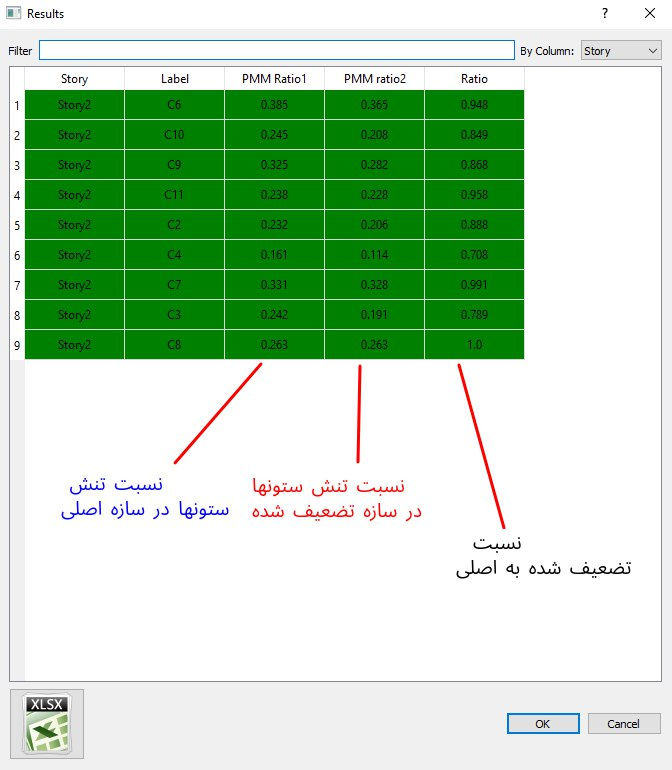
\includegraphics[scale=.7]{figures/weakness_column}
    \caption{جدول نسبت تنش ستونها در سازه اصلی و سازه تضعیف شده}
    \label{pic:weakness_column}
\end{figure}

\begin{figure}[H]
    \centering
    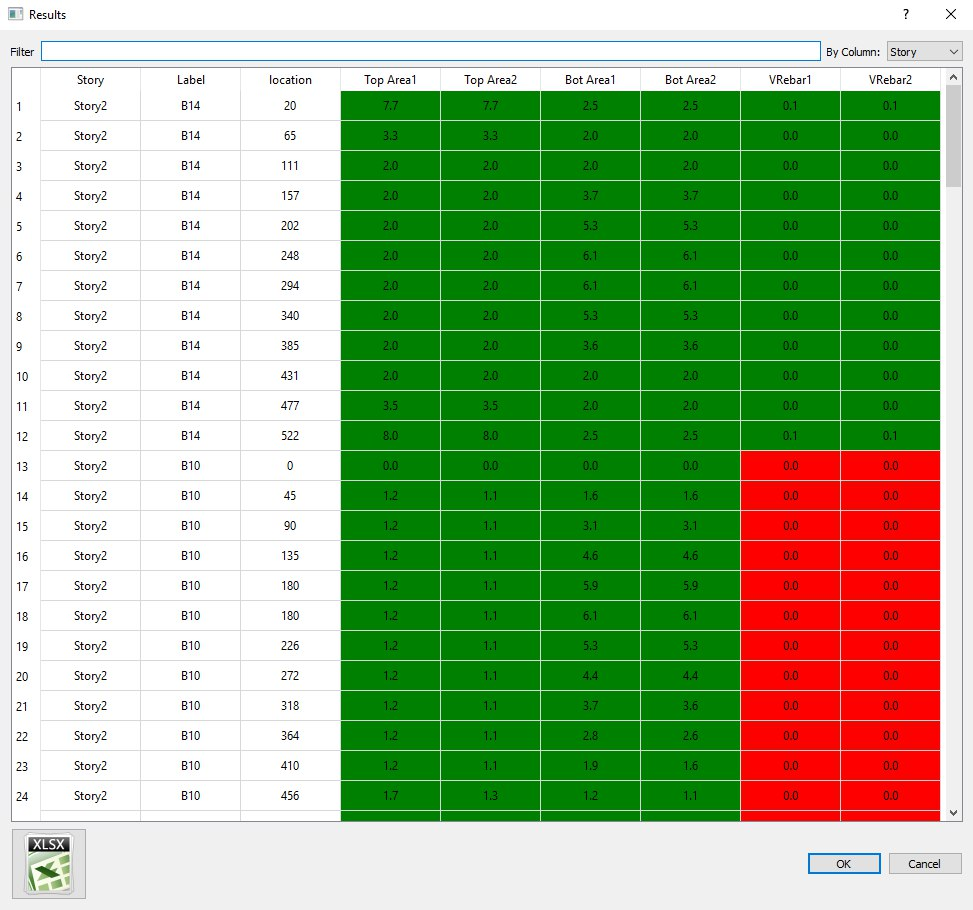
\includegraphics[scale=.6]{figures/weakness_beam}
    \caption{جدول مساحت میلگرد تیرها در سازه اصلی و سازه تضعیف شده}
    \label{pic:weakness_beam}
\end{figure}

\subsection{کنترل نامنظمی جرمی}
با کلیک بر روی آیکن مربوط به جرم، شما میتوانید به راحتی نامنظمی جرمی در سازه را مطابق شکل 
\ref{pic:mass_irregularity}
بررسی کنید، طبقات بام و خرپشته نیازی به کنترل ندارند و اگر در جدول رنگ اونها قرمز باشه مشکلی نیست:

\begin{figure}[H]
    \centering
    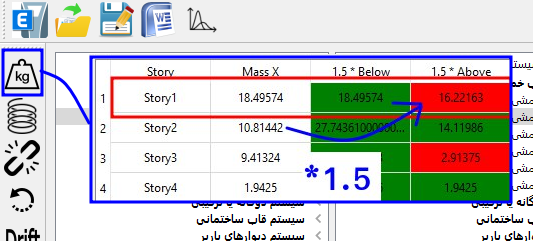
\includegraphics[scale=.7]{figures/mass_irregularity}
    \caption{کنترل نامنظمی جرمی}
    \label{pic:mass_irregularity}
\end{figure}

\section{نرم افزار مقاطع معادل}

بزودی ...

 \begin{figure}[H]
     \centering
     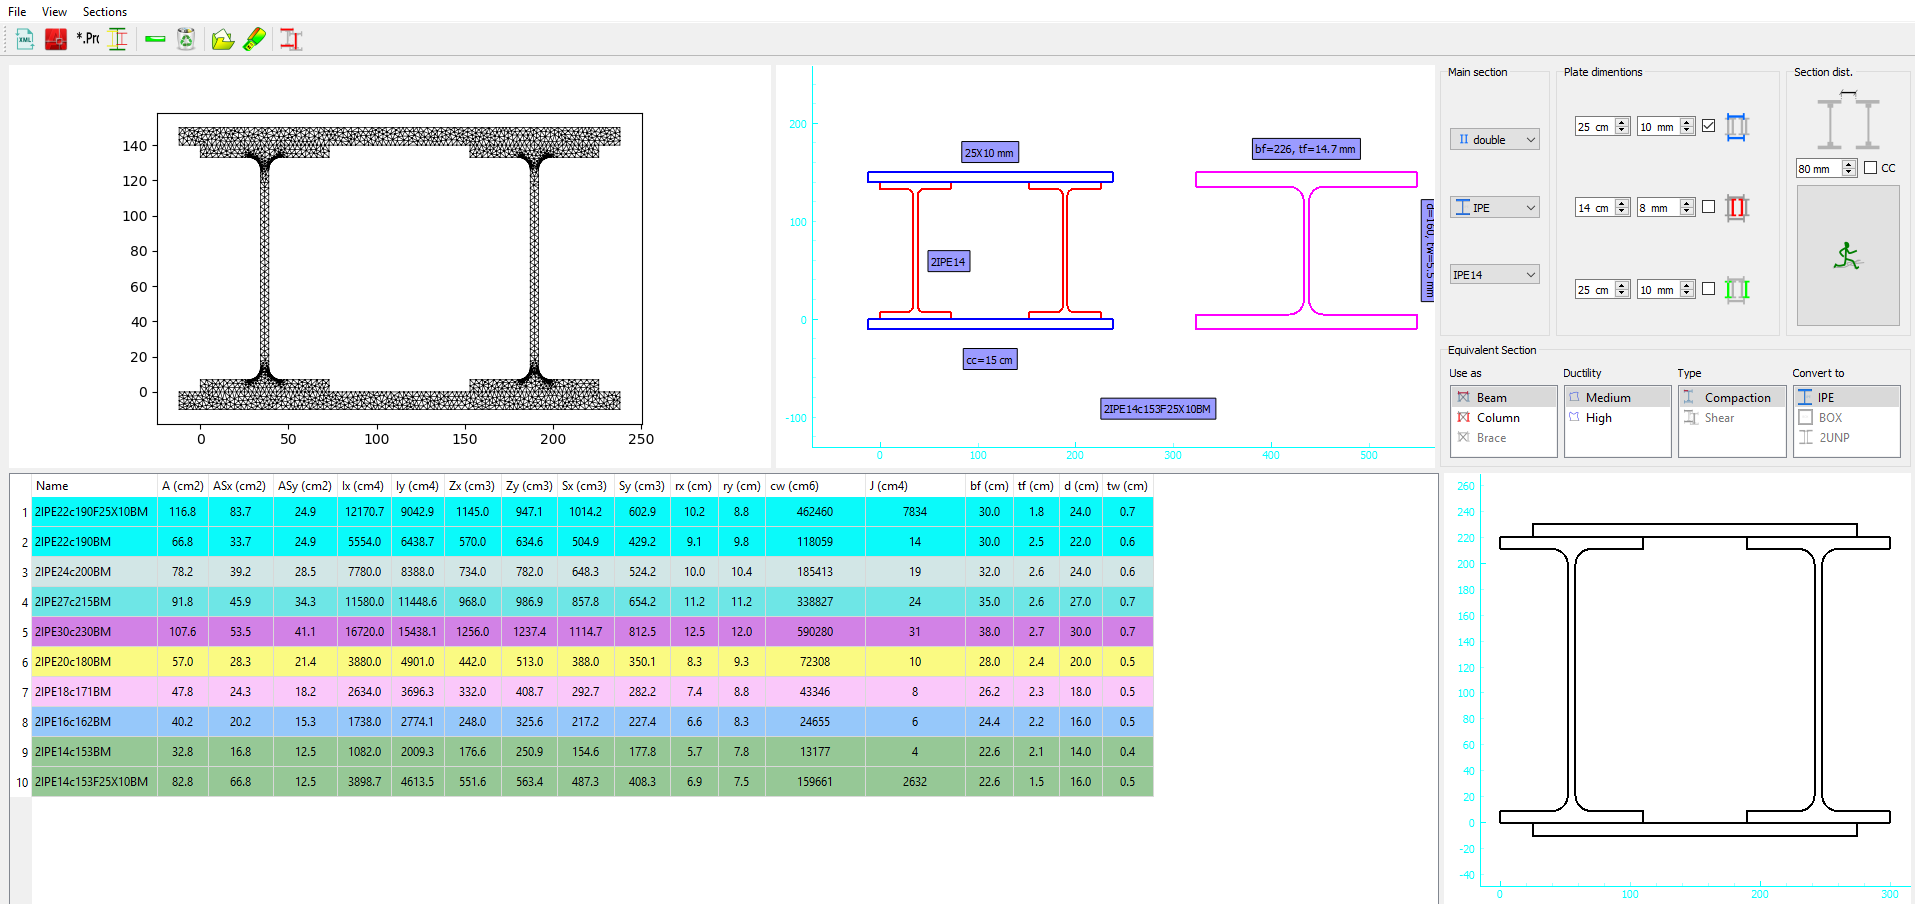
\includegraphics[scale=0.3]{figures/sections}
 \end{figure}
 

\section{فعال نمودن قابلیت ها}
در حال حاضر قابلیت های مختلف را میتوانید چند بار تست کنید. نرم افزار بعد از هر بار استفاده تعداد مجاز باقیمانده را به شما یادآوری میکند. بعد از اینکه این سقف تمام شد،
در صورت تمایل به استفاده، میتوانید مطابق پنچره راهنما (مطابق شکل 
\ref{pic:register}
) کدی که نرم افزار به شما میدهد را به همراه فیش واریزی، برای من ارسال کنید. من در اسرع وقت  قابلیت مورد نظر شما را فعال میکنم و به شما اطلاع میدهم. بعد از آن کافیست یکبار در حالی که به اینترنت متصل هستید قابلیت مورد نظرتان را اجرا کنید تا این قابلیت برای شما فعال شود.

 
 \begin{figure}
     \centering
     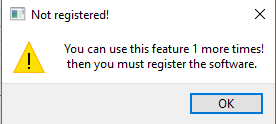
\includegraphics[scale=0.7]{figures/no_of_using}
     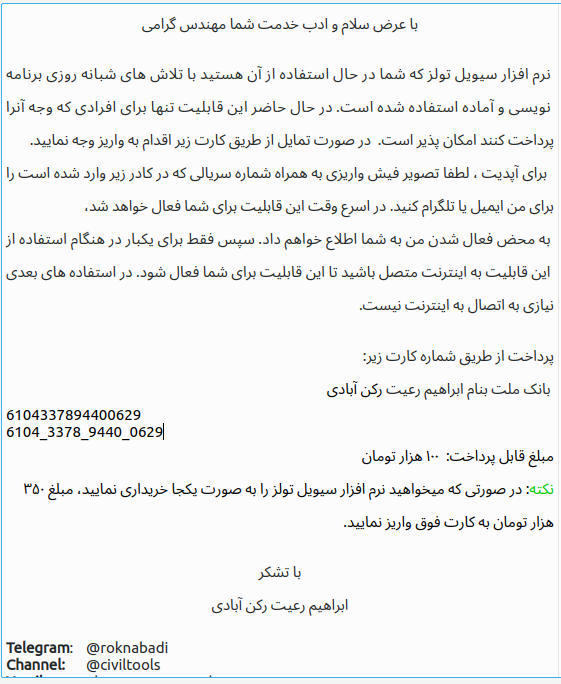
\includegraphics[scale=0.8]{figures/register}
     \caption{توضیح چگونگی فعال کردن قابلیت مورد نظر در نرم افزار}
     \label{pic:register}
 \end{figure}
 

% \input{export}
% \input{update}
% \input{faq}

% \end{twocolumn}
% \section{Combination of loads}
% \input{combinations.tex}
% \input{xc_design_technique.tex}

% \clearpage
% \input{appendix}

% \clearpage
% -----
%------------------------------------------------

%----------------------------------------------------------------------------------------
%	REFERENCE LIST
%----------------------------------------------------------------------------------------
%\phantomsection
%\nocite{OpenSeesManual,FeynmanVolI,Thomson}   % writes also non-cited references
% \nocite{*}
% \bibliography{jubail}  %file .bib 
% \bibliographystyle{plain} %normal style - listed in ABC order and labeled numerically
%\bibliographystyle{unsrt} %same as plain except entries appear in order of citation

% to compile the document run:
%    latex structural_design_report   to create the .aux file
%    bibtex structural_design_report  to get some of the citations and create a .bbl file
%    latex structural_design_report   again so that the cross references between latex file and bibliography
%                               are correct

%----------------------------------------------------------------------------------------

\end{document}
